\documentclass[12pt]{report}
\usepackage{graphicx}
\usepackage[a4paper, portrait, margin=2cm]{geometry}
\usepackage{listings}
\usepackage{array}

\lstset {
	breaklines=true,
	postbreak=+
}

\begin{document}
	\begin{center}
	\hspace{0pt}
	\vfill
		\vspace{50pt}
		\begin{Huge}
			\textbf{PROJECT REPORT}
		\end{Huge}
		\\
		\vspace{30pt}
		\begin{huge}
			EC302 - VLSI DESIGN LAB
		\end{huge}
		\\
		\vspace{30pt}
		\begin{Large}
			COMPILED BY \\ \vspace{3pt} AKASH A, NAVRATAN AND ANAND KUMAR SINGH \\ \vspace{11pt} ROLL NUMBERS : 191EC102, 191EC133, 191EC104
		\end{Large}
		\\
		\vspace{30pt}
		\begin{Large}
			PROFESSOR INCHARGE : DR. RAMESH KINI M
		\end{Large}
		\\
		\vspace{30pt}
		
\includegraphics[width = 10cm, height = 8cm]{NITK-Surathkal}
		\\
		\begin{large}
			NATIONAL INSTITUTE OF TECHNOLOGY KARNATAKA SURATHKAL
		\end{large}
	\vfill
	\hspace{0pt}
	\end{center}
	
	\newpage
	
	\begin{center}
		\begin{Large}
			Four Bit Signed Two's Complement Multiplier
		\end{Large}
	\end{center}
	\vspace{10pt}
	\begin{flushleft}
		\begin{Large}
			\textbf{OBJECTIVES}
		\end{Large}
	\end{flushleft}
	The project aims to perform the design, layout and characterization of a 4 bit multiplier in two's complement form. The multiplier takes in two 4-bit numbers (could be signed or unsigned) in two's complement form and the result is the product of the two numbers which is an 8-bit two's complement number.
	\vspace{3pt}
	\begin{flushleft}
		\begin{Large}
			\textbf{CIRCUIT DIAGRAM}
		\end{Large}
	\end{flushleft}
	\begin{center}
	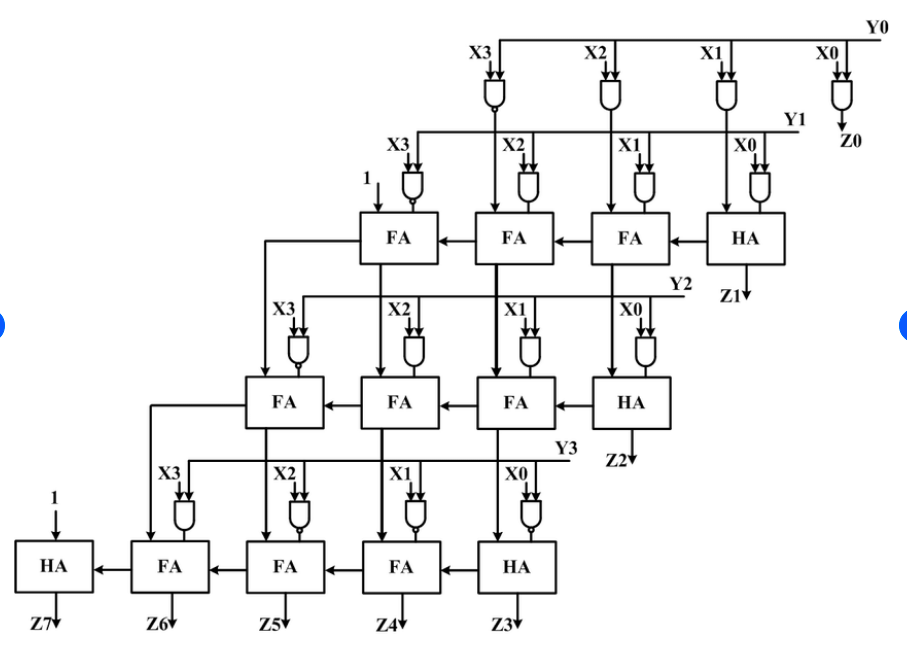
\includegraphics[height=12cm, width=15cm]{CircuitDiagram}
	\end{center}
	\vspace{3pt}
	\begin{flushleft}
		\begin{Large}
			\textbf{DESCRIPTION OF DESIGN}
		\end{Large}
	\end{flushleft}
	There are 3 main methods for multiplying binary numbers in 2's complement representation: shift-and-add method, Booth/Wallace method and array method. In this project, the array method of multiplication has been implemented which is the simplest and has the advantage of being easily pipelined for higher performance. \par The formula for multiplication of binary arguments expressed as sums of products of bit values and weights of positions in the 2's complement representation can be transformed, through appropriate term grouping and introduction of bit complements, to the form, which is a basis for constructing an array multiplier composed of elementary adders, shown in the figure above. In the array of elementary adders so many rows appear how many bits are in the number that are multiplied. On the inputs of the initial layer of elementary adders and to carry inputs at lower levels, appropriate logical products are supplied of multiplicand and multiplier bits (simple and complemented). The results of elementary additions (sum and carry bits) are supplied on inputs of adders in lower layers or they constitute already result bits, depending on the position of a given adder in the array.
	\begin{flushleft}
		\begin{Large}
			\textbf{IMPLEMENTATION DETAILS}
		\end{Large}
	\end{flushleft}
The RTL was designed using standard cells precreated using the technology file $pharosc.tech$. For the layout, over the cell routing technique was used as far as possible with some feedthroughs included for the sake of providing space for wiring. This helped in save space and create the circuit in a smaller area. For intra-cell routing, metal layer M1 was used while metal layers M2 and M3 were used for inter-cell routing. Top metal i.e. metal 3 in this case was used for the $V_{DD}$ and $V_{SS}$ rails to avoid the ground bounce problem since top metals have lesser resistance.\\
\vspace{2pt}
\begin{flushleft}
\textbf{Cells Used}
\end{flushleft}
a) Two input AND Gate to generate partial products and to generate carry for half adder
\begin{center}
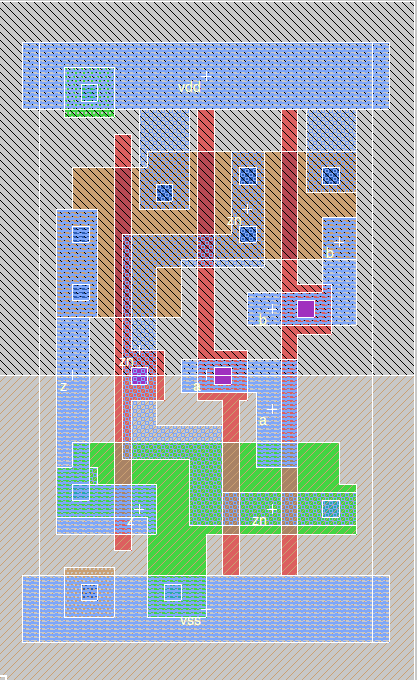
\includegraphics[height=8cm, width=8cm]{ANDcell}
\end{center}
b) Two input NAND gate for signed partial products
\begin{center}
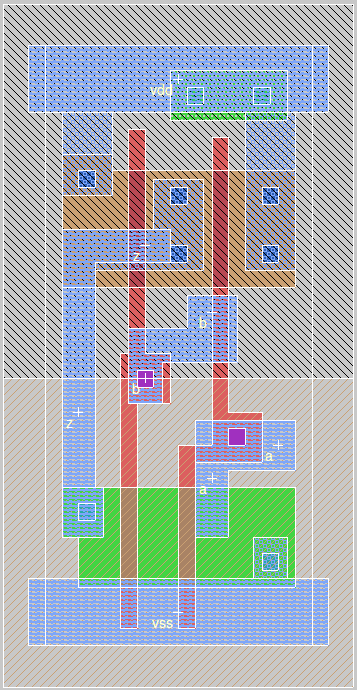
\includegraphics[height=8cm, width=8cm]{NANDcell}
\end{center}
\newpage
\begin{flushleft}
c) Two input XOR gate for half adder
\end{flushleft}
\begin{center}
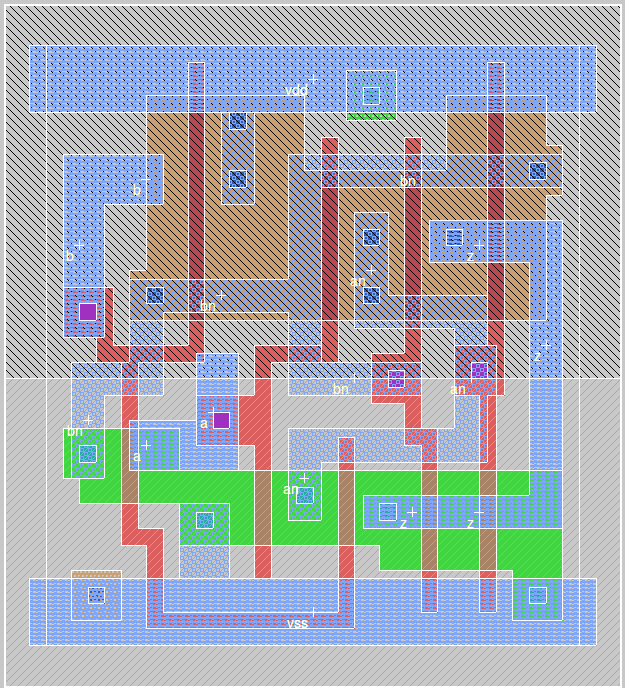
\includegraphics[height=7cm, width=8cm]{XOR2cell}
\end{center}
d) Three input XOR gate for full adder
\begin{center}
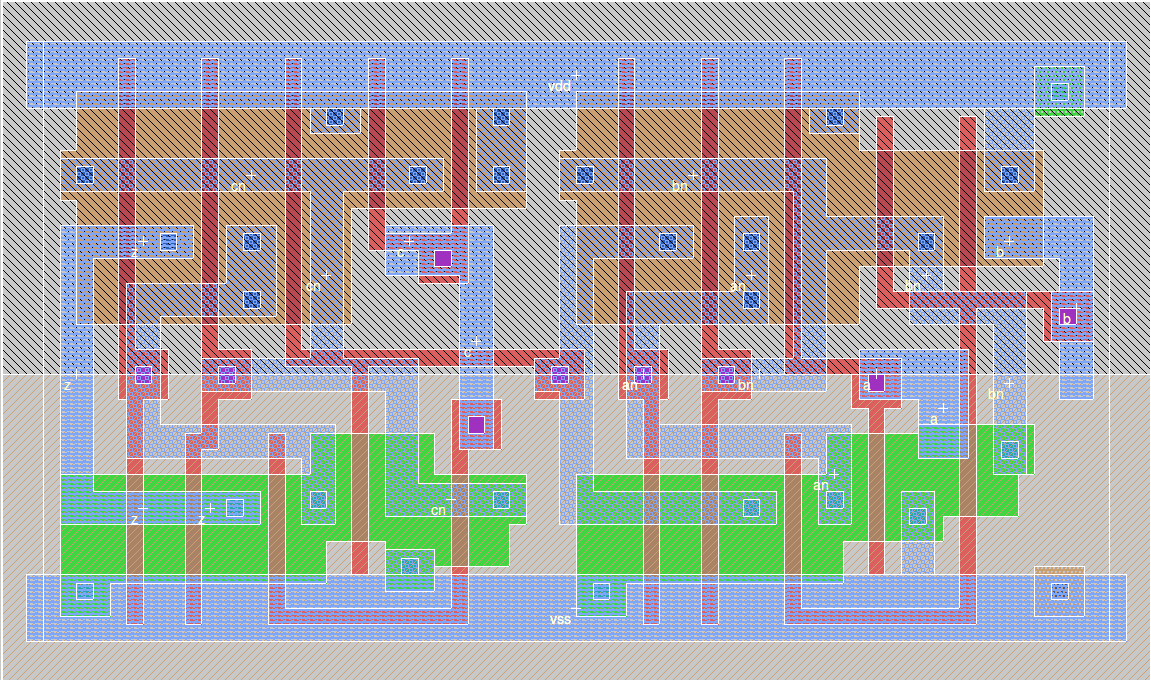
\includegraphics[height=8cm, width=8cm]{XOR3cell}
\end{center}
e) Three input carry generator to generate full adder carry
\begin{center}
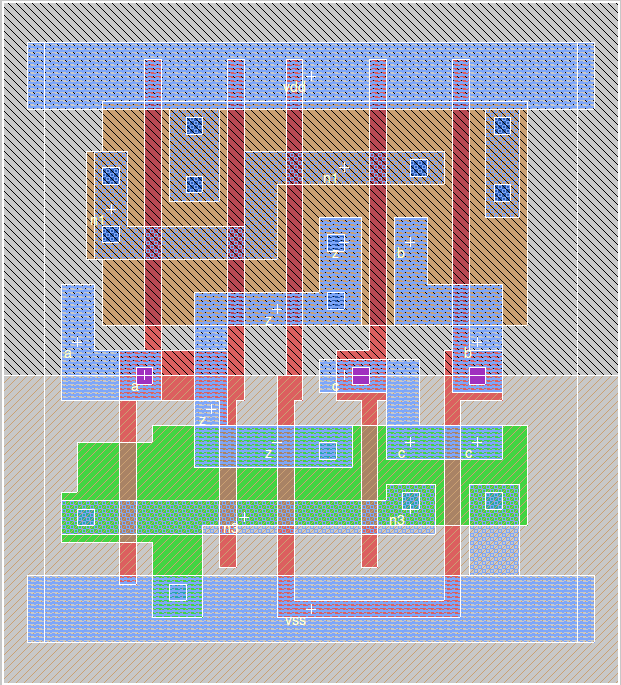
\includegraphics[height=7cm, width=8cm]{CGIcell}
\end{center}
f) Inverter to invert output of carry generator
\begin{center}
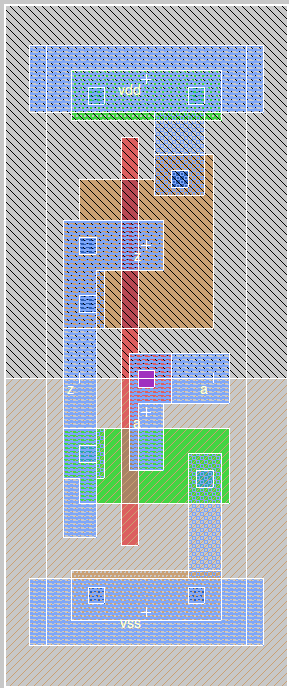
\includegraphics[height=8cm, width=8cm]{INVcell}
\end{center}
\vspace{3pt}
	\begin{flushleft}
		\begin{Large}
			\textbf{TOP LEVEL LAYOUT}
		\end{Large}
	\end{flushleft}
\begin{center}
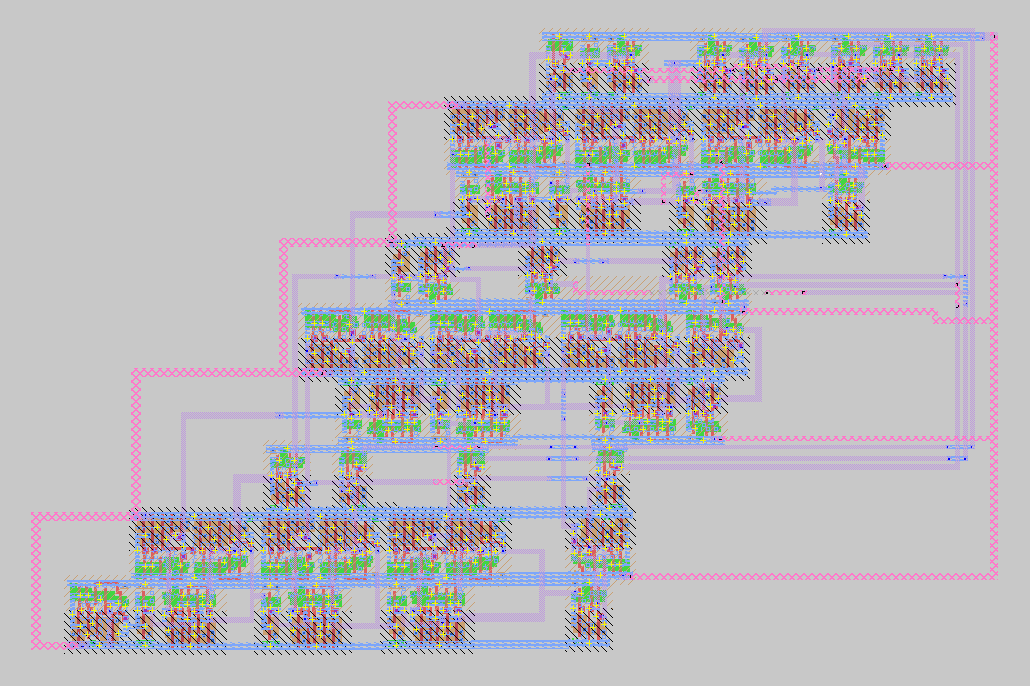
\includegraphics[height=12cm, width=15cm]{Layout}
\end{center}
Total Number of Cells = 52 \\
Area = (186+829)*(151+496) = 656,705 sq. microns
\newpage
	\begin{flushleft}
		\begin{Large}
			\textbf{TEST STRATEGY}
		\end{Large}
	\end{flushleft}
IRSIM, a circuit level simulation software was used to test the created .sim file for accuracy. In order to verify if the created circuit is correct, it was essential to test it for all possible binary numbers from 0000 to 1111 i.e. all possible four-digit binary numbers. The following python script can be used to generate all possible 4-digit binary numbers which henceforth needed to be permuted with itself to obtain the actual simulation test vextors for the two four-digit binary numbers.
\begin{lstlisting}
def printTheArray(arr, n):
 
    for i in range(0, n):
        print(arr[i], end = " ")
     
    print()
 
# Function to generate all binary strings
def generateAllBinaryStrings(n, arr, i):
 
    if i == n:
        printTheArray(arr, n)
        return
     
    # First assign "0" at ith position
    # and try for all other permutations
    # for remaining positions
    arr[i] = 0
    generateAllBinaryStrings(n, arr, i + 1)
 
    # And then assign "1" at ith position
    # and try for all other permutations
    # for remaining positions
    arr[i] = 1
    generateAllBinaryStrings(n, arr, i + 1)
 
# Driver Code
if __name__ == "__main__":
 
    n = 4
    arr = [None] * n
 
    # Print all binary strings
    generateAllBinaryStrings(n, arr, 0)
\end{lstlisting}
\newpage
	\begin{flushleft}
		\begin{Large}
			\textbf{WAVEFORM}
		\end{Large}
	\end{flushleft}
\begin{center}
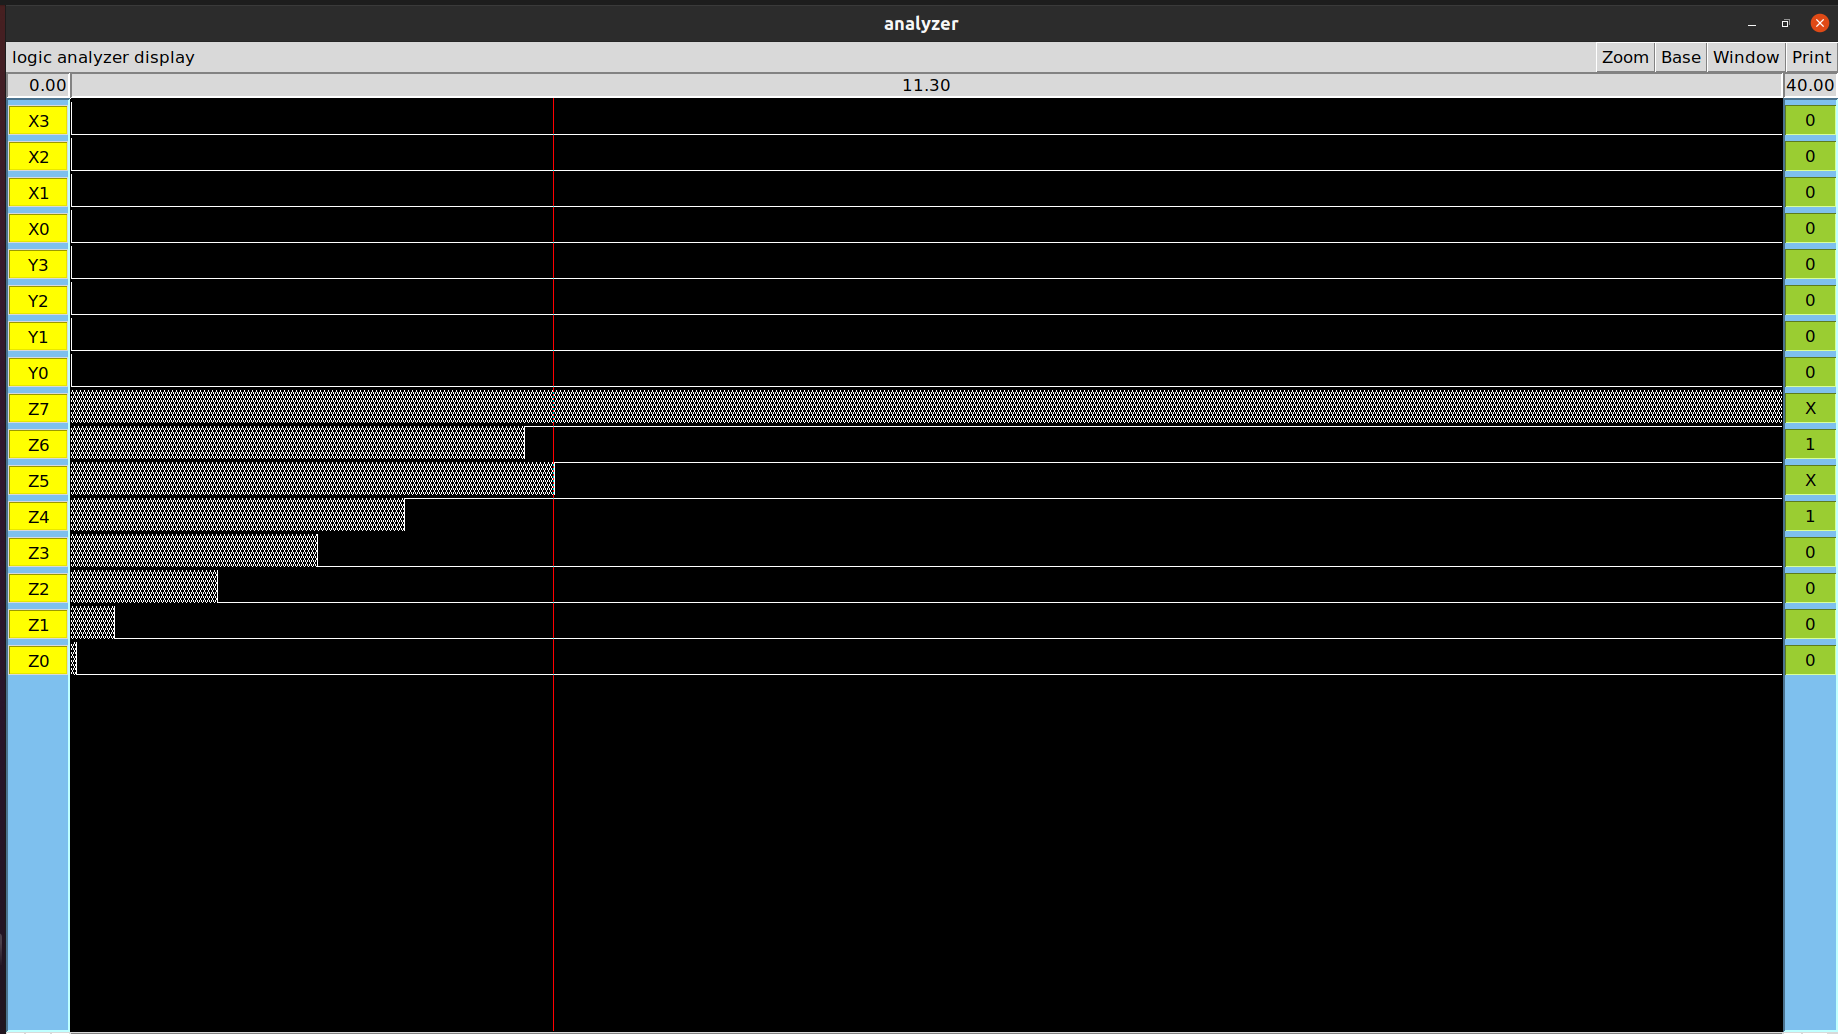
\includegraphics[height=12cm, width=15cm]{Waveform}
\end{center}
\vspace{4pt}
	\begin{flushleft}
		\begin{Large}
			\textbf{CONCLUSION}
		\end{Large}
	\end{flushleft}
We observe that the results obtained are not exactly as we might have expected. There are some errors which are obtained. This can be attributed to bad layout practices since odd metal layers were run vertically and horizontally and same was true for even metal layers. Another reason could have been the lack of a modular approach in the design. These are two things that could have been improved on and could have given the correct result if followed.
\end{document}